
\documentclass[a4paper,11pt,twoside]{scrartcl}
\usepackage[utf8x]{inputenc}
\usepackage{graphicx}
\usepackage{geometry}
\usepackage[ngerman]{babel}
%\usepackage{babelbib}
%\usepackage[backend=biber]{biblatex}
\usepackage{units}
\usepackage{url}
\usepackage{setspace}
\usepackage[
	pdftitle={Energie_Suffizienz},
 	pdfauthor={et.al.},
% 	pdfsubject={},
% 	pdfkeywords={},
	pdfstartview=FitH, % Auf Seitenbreite anpassen (Anzeige)
	pdfborder={0 0 0},
%  	bookmarks=true,
% %	plainpages=false,
	colorlinks=false,
	hyperfootnotes=false,
	pagebackref=false]{}
\usepackage[colorinlistoftodos,prependcaption,textsize=normalsize]{todonotes}  % disable
\usepackage{amsmath}
\usepackage{amstext}
\usepackage{amssymb}
\usepackage{color}
\usepackage[numbers]{natbib}
\usepackage{pdfpages}
\usepackage{hyphenat}
\usepackage{pdflscape} % für drucken ändern auf package lscape /pdflscape
\usepackage{textpos}
\usepackage{microtype}
\usepackage{enumitem}
\usepackage{multirow}
\usepackage{pdfcomment}

\usepackage{pgfgantt} % gantchart für den Arbeitsplan

% \usepackage{hyphenat}
\usepackage{float}
\usepackage{placeins}
\RequirePackage[bf]{caption}

\renewcommand{\textfraction}{.01} % vorher: .2
\renewcommand{\floatpagefraction}{.99}% vorher: .5
\renewcommand{\topfraction}{0.9}	% max fraction of floats at top
\renewcommand{\bottomfraction}{0.9}	% max fraction of floats at bottom

\newcommand{\ltab}{\raggedleft\arraybackslash}
\newcommand{\ctab}{\centering\arraybackslash} 
\newcommand{\rtab}{\raggedright\arraybackslash}

\usepackage{tabularx}
\newcolumntype{L}[1]{>{\raggedright\arraybackslash}p{#1}} % linksbündig mit Breitenangabe
\newcolumntype{C}[1]{>{\centering\arraybackslash}p{#1}} % zentriert mit Breitenangabe
\newcolumntype{R}[1]{>{\raggedleft\arraybackslash}p{#1}} % rechtsbündig mit Breitenangabe

\newcommand{\rem}[1]{}

% \renewcommand{\figurename}{Abb.}
% \renewcommand{\tablename}{Tab.}

\usepackage{acronym}
%\renewcommand{\bflabel}[1]{\normalfont{\normalsize{#1}}\hfill}

\usepackage[automark]{scrpage2}
\pagestyle{scrheadings}
\clearscrheadfoot
\ohead{\headmark}
\ofoot{\pagemark}
\setheadsepline{0.4pt}
\setfootsepline{0.4pt}

\setkomafont{pageheadfoot}{\rmfamily\small}

\renewcommand{\thefigure}{\arabic{section}-\arabic{figure}}
\renewcommand{\thetable}{\arabic{section}-\arabic{table}}

\newcommand{\entspricht}{\mathrel{\widehat{=}}}

\geometry{left=25mm,right=25mm, top=28mm, bottom=28mm}
\parindent 0pt
\parskip 11pt

% kein Platz zwischen \items
\setlist{nosep}
% Platz nach Überschriften reduzieren
\usepackage{titlesec}
\titlespacing*{\section}{0pt}{0pt}{0pt}
\titlespacing*{\subsection}{0pt}{0pt}{0pt}
\titlespacing*{\subsubsection}{0pt}{0pt}{0pt}
\titlespacing*{\paragraph}{0pt}{0pt}{5pt} % horizontal spacing in paragraph

\begin{document}
\onehalfspacing

\clearpage


{\singlespacing

\thispagestyle{empty}
\begin{center}

%first row logos
\begin{figure}[htb]
    \centering
    \begin{minipage}[c]{0.3\linewidth}
        \centering
        
\includegraphics[width=4.5cm]{logos/europa-universitaet-flensburg-hauptlogo-rgb-600dpi.png}
    \end{minipage}
    \hfill
    \begin{minipage}[c]{0.35\linewidth}
        \centering
        \includegraphics[width=5cm]{logos/Logo_interdiszi_institut.png}
    \end{minipage}
    \hfill
    \begin{minipage}[c]{0.3\linewidth}
        \centering
        \includegraphics[width=2.5cm]{logos/Logo_wuppertal.png}
    \end{minipage}
\end{figure}

\iffalse
%second row logos
\begin{figure}[htb]
    \centering
    \begin{minipage}[c]{0.3\linewidth}
        \centering
        \includegraphics[width=2.2cm]{logos/2015_Logo_TUM_RGB.jpg}
    \end{minipage}
    \hfill
    \begin{minipage}[c]{0.35\linewidth}
        \centering
        \includegraphics[width=5.5cm]{logos/isea_rwth_logo.jpg}
    \end{minipage}
    \hfill
    \begin{minipage}[c]{0.3\linewidth}
        \centering
        \includegraphics[width=3cm]{logos/TU_Logo_lang_RGB_rot.png}
    \end{minipage}
\end{figure}
\fi
\vspace*{1 cm}

{\LARGE\textbf{\textsf{Skizze Nachwuchsforschungsgruppe}}

\textsf{\textit{im Rahmen der Bekanntmachung \glqq inter- und transdisziplinär arbeitende Nachwuchsgruppen im Rahmen der Sozial-ökologischen Forschung\grqq} }
}

\vspace{0.5cm}

{\Huge
\textbf{\textsf{Die Rolle von Energie-Suffizienz in Energiewende und Gesellschaft}}

\textbf{\textsf{}}
}

{\Huge
\textbf{\textsf{Akronym:{EnSufGe}}}
}

\vspace{1cm}

Eingereicht durch
Frauke Wiese\\
i$^{2}$ Interdisziplinäres Institut für Umwelt-, Human- und Sozialwissenschaften\\
Europa-Universität Flensburg, Auf dem Campus 1, 24943 Flensburg


\vspace{0.5cm}

An den Projektträger im DLR \\
AE 41 Globaler Wandel/Klima- und Umweltschutz, Sozial-ökologische Forschung \\
Heinrich-Konen-Straße 1, 53227 Bonn


\end{center}
\iffalse
\begin{table*}[b]
\centering
\footnotesize
\begin{tabular}{ | p{5cm} | p{5cm} |} \hline
\textbf{Konsortialpartner} & \textbf{Modelle/Frameworks} \\ \hline
Reiner Lemoine Institut & Leitung des Experiments \\ \hline
Technische Universität München & urbs \\ \hline
Europa-Universität Flensburg & oemof \\ \hline
RWTH Aachen & GENESYS-2 \\ \hline
Technische Universität Berlin & OSeMOSYS \\ \hline
Dänische Technische Universität & Balmorel \\ \hline
\end{tabular}
\label{tab:Partner}
\end{table*}
\fi


\clearpage
}

\setcounter{page}{1}

\section{Zielstellung und gesellschaftlicher Bedarf}
%\textit{Beschreibung der Problem- und Zielstellung sowie des gesellschaftlichen Bedarfs}

Klimawandel, Ressourcenverknappund und zunehmende Umweltveränderungen lassen die Transformation des Energiesystems zu einer der der zentralen gesellschaftlichen Herausforderungen werden. Noch ist weitgehend offen, wie die Versorgung mit Strom, Wärme, Mobilität sichergestellt werden kann, während Klimaziele erreicht, soziale Gerechtigkeit gewahrt und die natürlichen Grenzen unseres Planeten langfristig eingehalten werden können. 

Energiesystem-Modelle haben sich als Werkzeuge etabliert, um technisch mögliche und ökonomisch vorteilhafte Energiewende-Pfade darzustellen und zu analysieren. Sie helfen dabei, komplexe Zusammenhänge zwischen technischen Möglichkeiten (z.B. Flexibilität), Umweltbedingungen (z.B. Wetter-abhängige Erneuerbare), Marktregeln (z.B. Energy-only-Markt) im Licht klimapolitischer Zielsetzungen zu verstehen und unterstützen somit die Klima- und Energiepolitik.

Ein entscheidender Einflussparameter für berechnete Szenarien ist die zukünftige Nachfrage nach Strom, Wärme und Mobilität. Die Mehrzahl der bisherigen Modelle legt den Fokus  auf die Bereitstellung von Energiedienstleistungen. Die Nachfrage-Seite wird meist nur innerhalb enger Grenzen variiert. So berücksichtigen viele Modelle beispielsweise die Verschiebung der Nachfrage von fossilen Brennstoffen zu Strom durch die Elektifizierung im Wärme- und Transportsektor. Eine übergreifende Perspektive, welche die verschiedenen Bereiche berücksichtigt und integriert, in denen Energie gebraucht wird, steht noch aus. Zudem wird in den meisten Modellen die absolute Nachfrage nach Energie nicht in Frage gestellt. Mit anderen Worten: Bislang sind Modellierungen weitgehend blind gegenüber Veränderungen der Nachfrage nach Energie durch gesellschaftlichen Wandel oder Verhaltensänderungen.

Nicht nur in der Modellierung von Energiewende-Pfaden, sondern auch  bei Klimaschutz-Strategien liegt der Fokus bisher auf im weitesten Sinn technikorientierten Lösungen bei der Erzeugung und Distribution von Energie für Wohnen, Bauen, Ernährung und Mobilität \cite{Creutzig2018}. 

Zwar bieten laut Modellrechnungen Erneuerbare Energien und Effizienz die Möglichkeit im Jahr 2050 80-95 Prozent Treibhausgas-Reduktion in Deutschland \cite{BMWi2017} zu erreichen. Es gibt jedoch verschiedene Gründe keine der drei Nachhaltigkeitsstrategien Konsistenz, (Erneuerbare Energien ersetzen Fossile), Effizienz (relative Reduktion des Energieverbrauchs bei Bereitstellung der gleichen Energiedienstleistung) und Suffizienz (absolute Reduktion der Nachfrage nach Energiedienstleistungen durch veränderte soziale Praktiken und gesellschaftliche Leitbilder) außer Acht zu lassen: Zum einen setzten die ambitionierten Ziele des Pariser Klimaabkommens die Herausforderung nochmal auf eine neue Stufe \cite{Rogelj2018}. Außerdem sprechen Aspekte wie Flächenverbrauch (Referenz fehlt noch), Ressourcenbedarf (Referenz fehlt noch) und Akzeptanzfragen \cite{Fuchs2016}, zusammengefasst die Einhaltung der planetaren Grenzen \cite{Rockstroem2009} dafür, die Chancen die Suffizienz bietet, nicht zu übersehen \cite{SAMADI2017}.

Desweiteren ist bisher nicht abschließend geklärt, in welchem Ausmaß Emissionsreduktionen in Deutschland durch Konsistenz und Effizienz tatsächlich erreicht wurden. Verlagerungseffekte in andere Länder könnten ebenso eine Rolle gespielt haben \cite{Wiedmann2015}, so dass die Emissionsreduktionen bei Bilanzierung nach Verursacherprinzip geringer ausfallen. Auch die Rolle, die Effizienz spielen kann, ist nicht klar. Zielszenarien für Deutschland gehen von einer Reduzierung der Stromnachfrage durch eine massive Steigerung von Effizienz aus \cite{BMWi2017}. Zugleich findet jedoch in der fachwissenschaftlichen und energiepolitischen Diskussion der Befund Aufmerksamkeit, dass Energieeffizienzsteigerungen in der Regel von Rebound-Effekten begleitet werden, welche die Einsparungen teilweise kompensieren oder mitunter sogar zu einem verstärkten Energieverbrauch („Backfire“) führen \cite{DeutscherBundestag2013,Santarius2012}. Auch aufgrund solcher Rebound-Effekte wurden in den vergangenen Jahren die Energiesparpotenziale nicht voll ausgeschöpft, was dazu beitrug, dass in Deutschland trotz aller Maßnahmen zur Verbesserung der Energieeffizienz der Stromverbrauch im Jahr 2016 gegenüber 2008 (acht Jahre) um nur 1,5 Prozent gesunken ist \cite{UBA2017}. Dies lässt das erklärte Ziel weitere 8,5 Prozent bis 2020 (vier Jahre) zu schaffen sehr ambitioniert erscheinen.

In Anbetracht des möglichen Beitrags der Suffizienz und der Größe der Herausforderung, ist die Rolle von Energie-Suffizienz derzeit unterrepräsentiert in Diskussion und Forschung für Klimaschutz und Energiewende. Abbildung \ref{fig:zusammenspiel} verdeutlicht schematisch den Gedanken des Zusammenspiels der drei Dimensionen für die Erreichung der Klimaziele. 


\begin{figure}[!h]
    \centering
    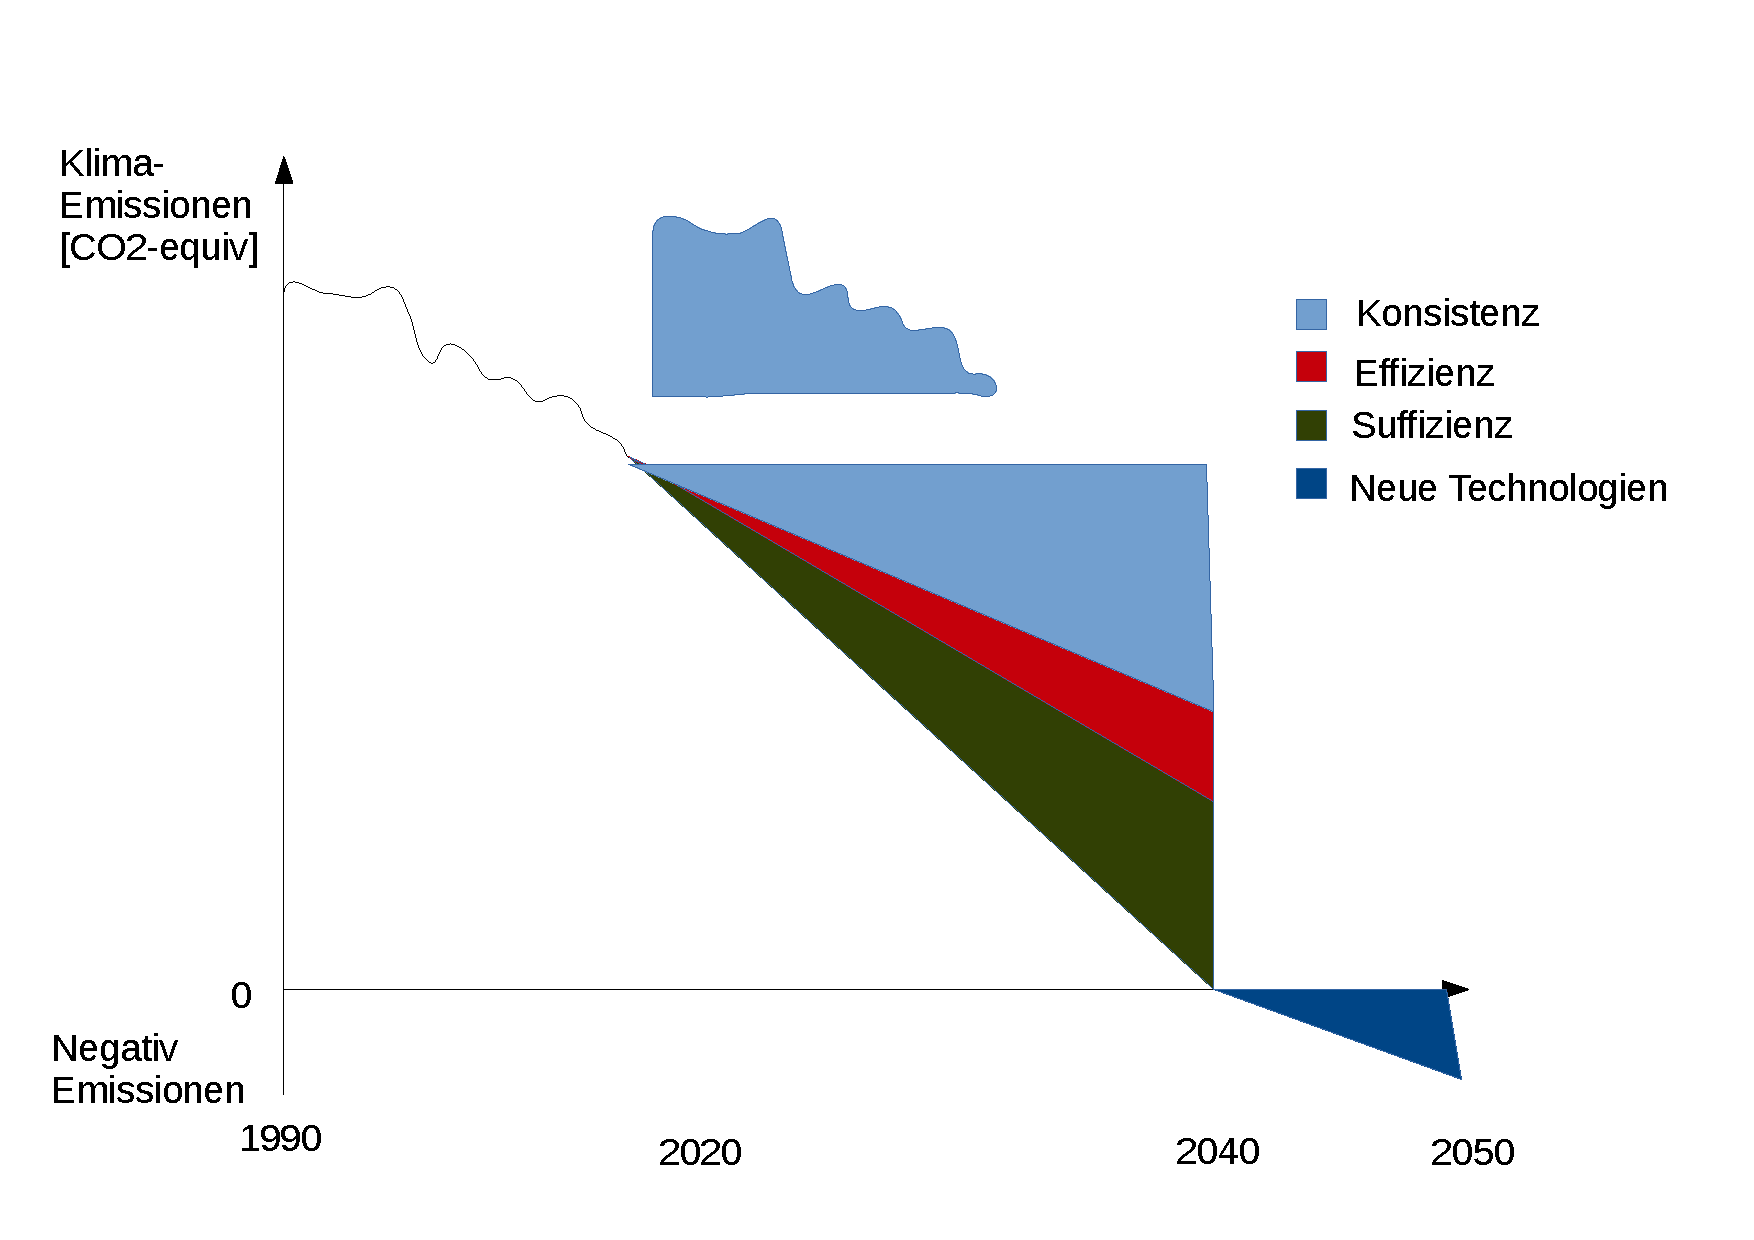
\includegraphics[width=0.8\textwidth]{figures/Zusammenspiel2.pdf}
    \caption{Schamatisch: Bisherige Emissionsreduktion durch Konsistenz (links), notwendiger Beitrag von Effizienz und Suffizienz in Zukunft (rechts) zur Erreichung der Klimaziele in Deutschland}
    \label{fig:zusammenspiel}
\end{figure}

Weiter hat sich in der Forschung die Erkenntnis durchgesetzt, dass nur unter Einbeziehung und dem Zusammenspiel verschiedener Disziplinen - wie technisch-/ingenieurwissenschaftlicher Fachrichtungen, Politik-, Wirtschafts- und Sozialwissenschaften - die gesellschaftliche Herausforderung der Transformation des Energiesystems erfolgreich bewältigen lässt \cite{WGBU2012}.

Besonders deutlich wird die Notwendigkeit der verstärkten interdisziplinären Zusammenarbeit bei der Erstellung von Energie-Szenarien. Gesellschaftliche Entwicklungen haben enormen Einfluss auf die Nachfrage nach Energie-Dienstleistungen, die politischen Rahmenbedingungen für die Erzeugungs- und Distributionswege sowie die technisch-ökonomischen Optionen zur Erfüllung der Energienachfrage (schematisch dargestellt in Abbildung \ref{fig:szenarien}). Gängige Praxis in der Energiesystem-Modellierung ist es, nur Letzteres in den Blick zu nehmen, gesellschaftliche Dynamiken hingegen weitgehend zu ignorieren.  Dieses Vorgehen erlaubt eine Abschätzung der Leitungsfähigkeit sozio-technischer Innovationen. Allerdings um den Preis einer Vorstellung, die Gesellschaft als mehr oder weniger statisches Konstrukt imaginiert und nicht als das hoch dynamische, beständigen Veränderungen unterworfene Gemeinwesen, das sie ist.   (Abbildung \ref{fig:szenarien} links). Für konsistente und damit belastbare Energie-Szenarien ist die Integration sozialwissenschaftlicher Wissensbestände in Bezug auf künftig zu erwartende gesellschaftliche Transformationsprozesse und ihre Auswirkungen auf den gesellschaftlichen Metabolismus unverzichtbar. Beispielhaft seien hier die Digitalisierung oder der demografische Wandel genannt. Beide Prozesse werden mit hoher Wahrscheinlichkeit Auswirkungen auf die Nachfrage nach Energiedienstleitungen haben, in welchem Umfang und in welche Richtung - steigende oder sinkende Nachfrage - ist erstens kontingent und zweitens allein mit Verweis auf die Leistungsfähigkeit technischer Innovationen nicht zu beantworten. Noch nicht abzusehen ist auch, in welchem Ausmaß etwa kommunale und nationale Klimaschutzmaßnahmen - erinnert sei hier an die aktuelle Diskussion um den ticketlosen ÖPNV - soziale Innovationen oder einen Wandel gesellschaftlicher Werte und Normen beeinflussen werden. (Abbildung \ref{fig:szenarien} rechts). Außerdem ermöglicht die Erweiterung des Bezugsrahmen um die gesellschaftliche Perspektive, Suffizienz neben Effizienz und Konsistenz in der Modellierung abzubilden. 

\begin{figure}[!h]
    \centering
    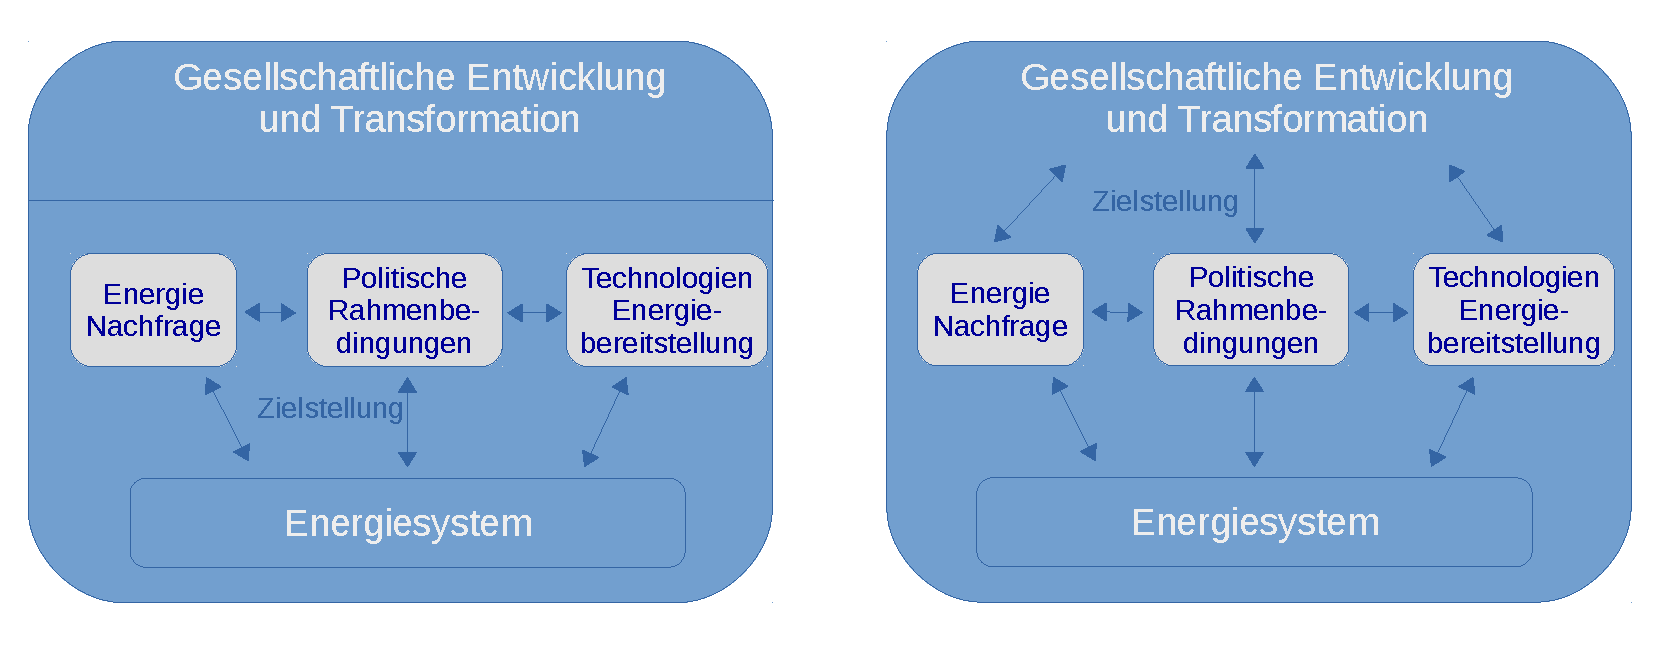
\includegraphics[width=0.8\textwidth]{figures/Szenarien.pdf}
    \caption{Rahmen für Energie-Szenarien: Links: Getrennte Betrachtung / Rechts: Einbettung der Annahmen für Energie-Nachfrage, Politikrahmen und technische Optionen in gesellschaftliche Entwicklungen}
    \label{fig:szenarien}
\end{figure}

Ziele der Nachwuchsforschungs-Gruppe Energie-Suffizienz sind:
\begin{itemize}
 \item Einen in der bisherigen Diskussion um die Transformation des Energiesystems in Richtung Nachhaltigkeit unterrepräsentierten Aspekt  -- Suffizienz -- intensiv dahingehend zu erforschen
  \item In der interdisziplinäre Kooperation ein Verfahren für die Erstellung von konsistenten, multiperspektivischen  Energieszenarien zu entwickeln und zu erproben
  \item (Weiter)-Entwicklung eines Energiesystem-Modells, in dem Konsistenz, Effizienz und Suffizienz integriert betrachtet werden können
 \item Einen möglichen und eventuell notwendigen Beitrag von Energie-Suffizienz zur Erreichung der Klimaziele auf nationaler (Deutschland) und kommunaler (Flensburg) Ebene ermitteln
 \item Die Entwicklung von Zukunftsszenarien zur Transformation des Energiesystems in Richtung Nachhaltigkeit 
 \item Die historische Rekonstruktion der Wechselwirkung zwischen Energiesystemtransformation und gesellschaftlichem Wandel  
 \item Handlungsoptionen für Suffizienz-Politik von kommunaler bis EU-Ebene
 \item Literatur und Methoden der Energiesystem-Analyse als auch die der sozial-ökologischen Transformationsforschung erweitern. Schwerpunkt liegt dabei auf Synergien zwischen den Forschungsgebieten.
 \item Das Methodenspektrum junger Forscher mit Hintergründen aus Sozialwissenschaft (sozial-ökologische Transformationsforschung), Wirtschaftingenieurwesen (Energiesystem-Analyse) und Politikwissenschaft interdisziplinär erweitern
\end{itemize}

Im Rahmen des Projektes erarbeitete Daten und Software, werden open source zur Verfügung gestellt. Der Open Science Ansatz der der Nachwuchs-Forschunggruppe zugrunde liegen wird, beinhaltet auch den offenen Zugang zu Publikationen etc. Die Erkenntnisse sollen außerdem politische Entscheidungsprozesse zu Klimaschutz und Energiewende unterstützen und Empfehlungen für Suffizienzpolitik beinhalten. Ein Schwerpunkt wird die Ergebnis-Kommunikation auch im populär-wissenschaftlichen Bereich, um auch eine außerwissenschaftliche Öffentlichkeit zu erreichen.

\section{Stand von Wissenschaft und Technik sowie eigene Vorarbeiten}
\subsection*{Energiesystem-Analyse und Modellierung}
\begin{itemize}
    \item Energiesystem-Analyse und Modellierung: wichtige Rolle auch in policy advice, hochkomplexe Modelle, inzwischen auch Open Source Modelle, wenn auch noch Mangel an Transparenz
    \item Generelle Herausforderungen ESM:
    \begin{itemize}
     \item Open heißt nicht unbedingt verständlich, bisher Mangel an Ergebniskommunikation 
     \item Sozialwissenschaftlicher Komponenten bisher unterrepräsentiert wenn es auch auf dem Gebiet Akzeptanz
     \item Arbeiten im Bereich Energie-Nachfrage beziehen sich viel auf Flexibilität der Nachfrage, weniger auf die absolute Nachfrage nach Strom, Wärme, Mobilität
    \end{itemize}
    \item Eigene Vorarbeiten (Frauke): ESM, open ESM, kritische Betrachtung ESM, Verbindung über techn.-ökono. Sichtweise hinaus, bereits interdisziplinär gearbeitet / (EUM-Team): oemof, open, Klimaschutz (transdisziplinär)
\end{itemize}

\subsection*{Sozial-ökologische Transformationsforschung}
\textit{NEC: bitte ergänzen, v.a. in Bezug auf Energiewende und Suffizienz inklusive eigene Vorarbeiten}
% Rebound text von Bernd, siehe auch Bezug zu Nachwuchsgruppe Nachwuchsforschungsgruppe Rebound, Suffizienz und Digitalisierung)
    %https://www.fona.de/de/nachwuchsfoerderung-sozial-oekologische-forschung-20620.html
    %  1.05.2016 - 30.04.2021
    % Digitalisierung und sozial-ökologische Transformation. Rebound-Risiken und Suffizienz-Chancen digitaler Dienstleistungen
    
\subsection*{Sufizienz-Politiken}
\textit{Wuppertal: bitte ergänzen, v.a. in Bezug auf Energie-Suffizienz inklusive eigene Vorarbeiten}


\section{Bezug zur Sozial-ökologischen Forschung und zu den Förderzielen}

\url{https://www.fona.de/mediathek/pdf/SOEF_Foerderkonzept_barrierefrei.pdf}

SEHR GERN ERGÄNZEN

% Bezug zu sozial-ökologischer Forschung
%Ideen:
%interdisziplinäres Verständnis wird geschaffen und baut auf dem disziplinären Vorwissen auf indem teilweise gleiche Arbeitspaket erst disziplinär parallel ausgeführt werden um dann in der Synthesephase den gemeinsamen Blick drauf zu werden (z.B. Szenarien-Methoden)
%...gemeinsamen Methodenentwicklung vor dem Hintergrund transdisziplinärer Nachhaltigkeitsforschung....
% Kultur des interdisziplinären Veröffentlichen pflegen

% aus altem Antrag
Die Weiterentwicklung institutioneller Kapazitäten zur Durchführung transdisziplinärer Nachhaltigkeitsforschung wird durch die Verankerung der Nachwuchsgruppe am Interdisziplinären Institut für Umwelt-, Sozial und Humanwissenschaften an der Europa-Universität Flensburg geschaffen. In der eigenverantwortlichen Arbeitsgruppe bekommen junge Wissenschaftler*innen die Möglichkeit sich auf der Basis ihres disziplinären Vorwissens sozial-ökologischen Fragestellungen zu widmen. Möglichkeiten zur Weiterqualifizierung werden durch die  Nachwuchsgruppe für wissenschaftliche Mitarbeiter*innen geschaffen, die zwar schon jetzt an den Schnittstellen forschen, dafür aber nicht den entsprechenden Rahmen haben um sich auch wissenschaftlich zu qualifizieren.


\section{Forschungsarbeit, Arbeitsprogramm, Methoden, Disziplinen}
\textit{Beschreibung der geplanten Forschungsarbeiten und des Arbeitsprogramms, unter Einschluss der Darstellung von Methoden, die zur Anwendung kommen bzw. entwickelt werden sollen; sowie der disziplinären Zusammensetzung der geplanten Nachwuchsgruppe}

%%%%%%%%%%%

\begin{figure}[!h]
    \centering
    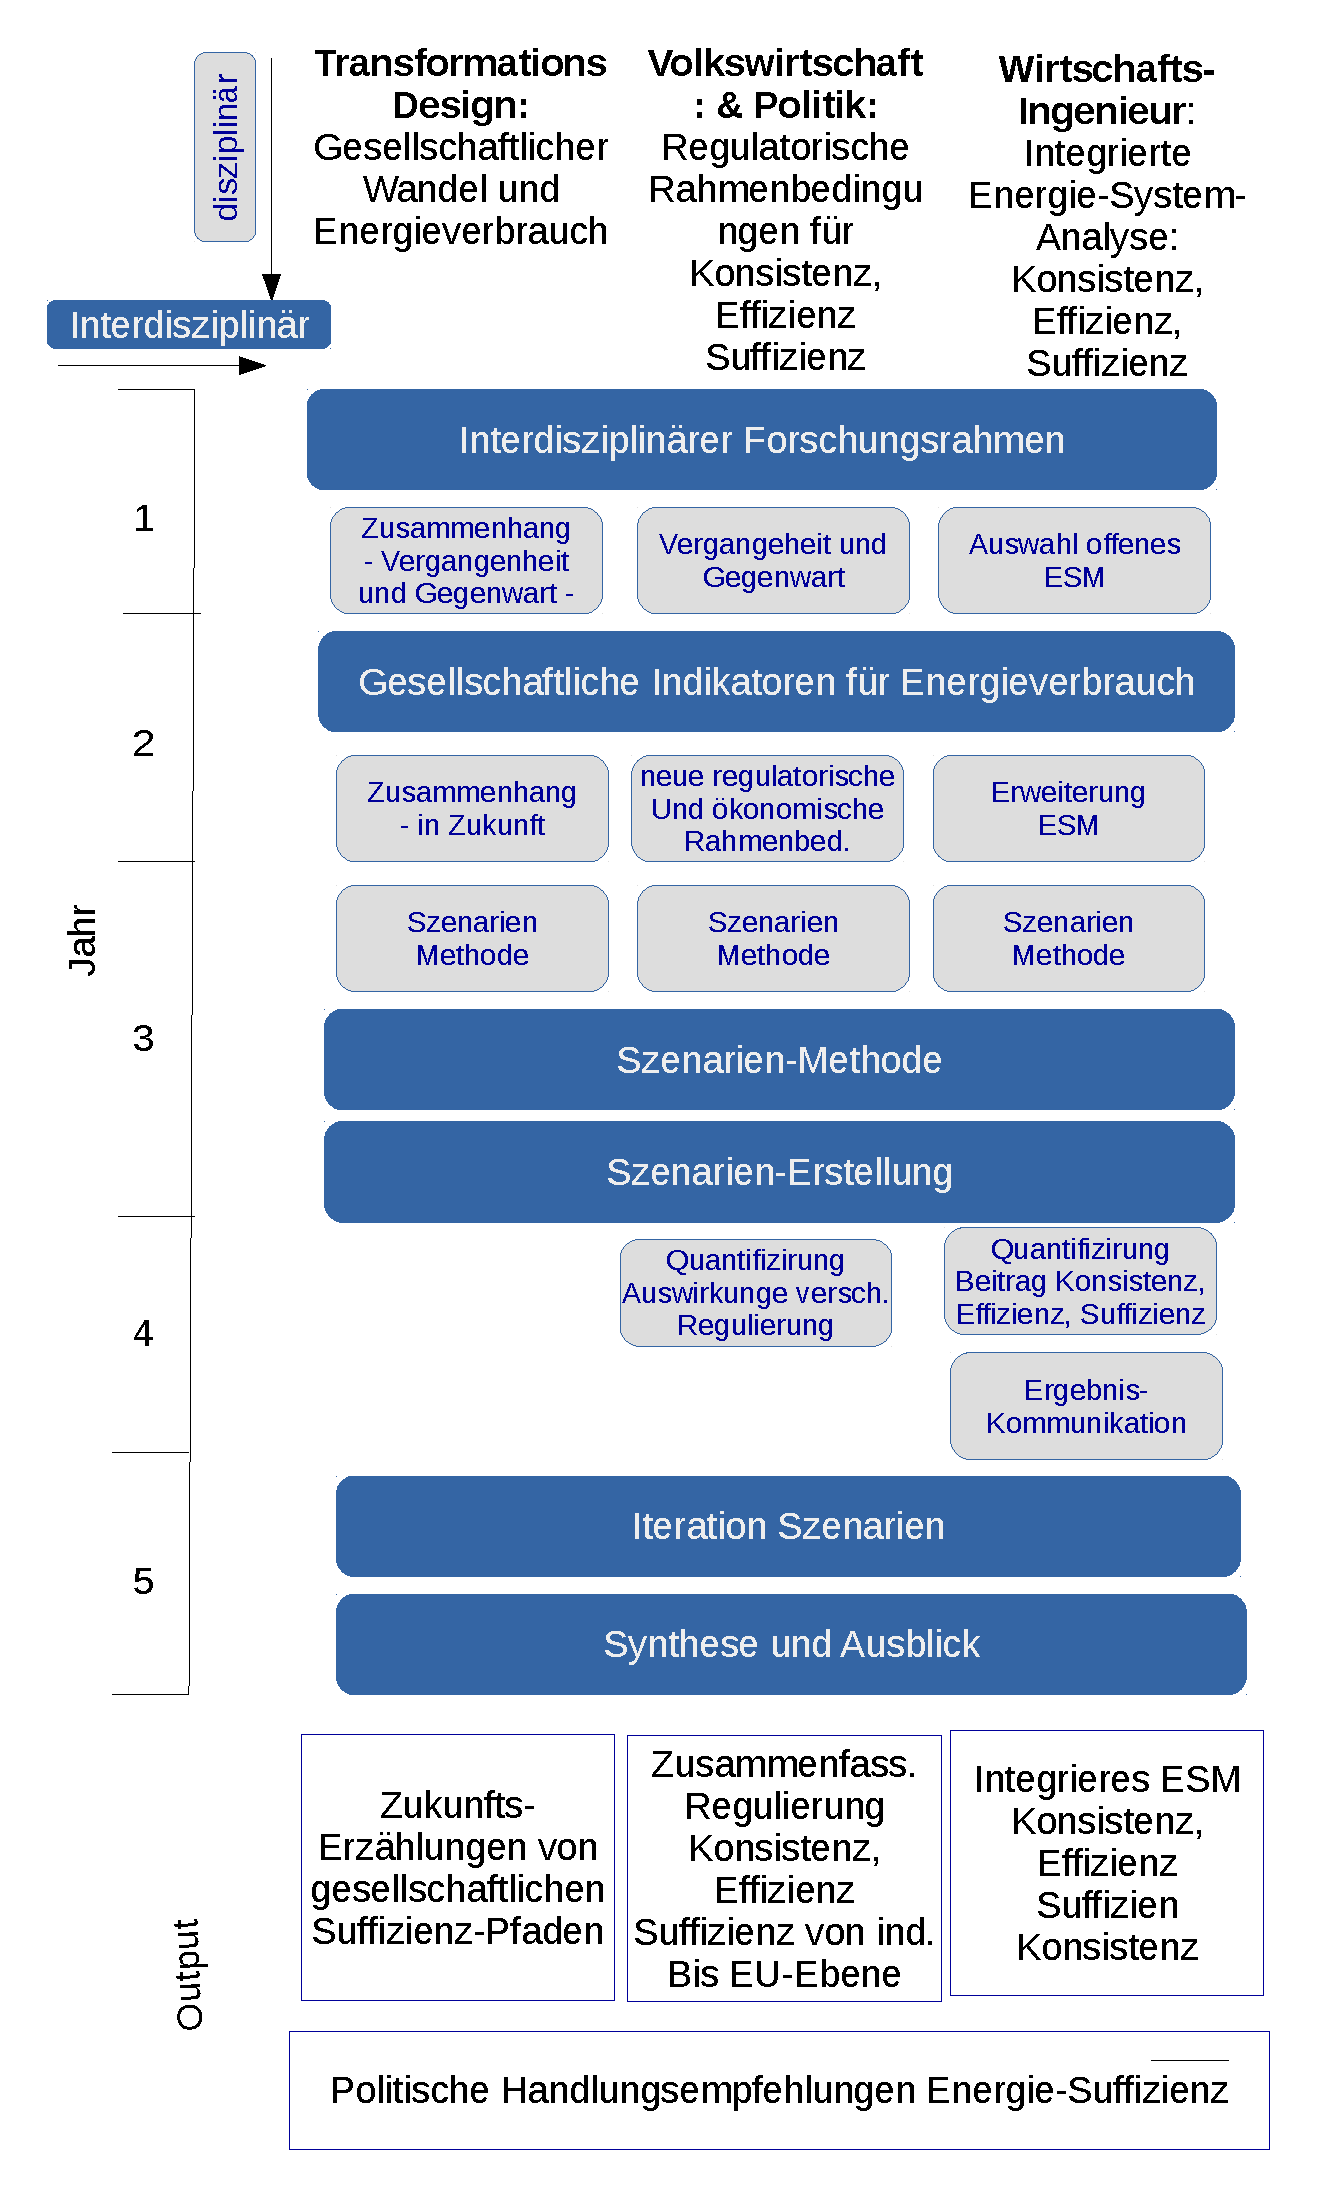
\includegraphics[width=0.8\textwidth]{figures/Forschungsarbeit.pdf}
    \caption{Forschungsprogramm: Disziplinäre Forschungsarbeit (vertikal) und  interdisziplinäre (horizontal) Arbeitspakete im Verlauf der fünf Jahre sowie geplanter disziplinärer und interdisziplinärer Output}
    \label{fig:forschungsprogramm}
\end{figure}

Abbildung \ref{fig:forschungsprogramm} gibt einen Überblick wie die disziplinären Forschungsfelder (vertikal dargestellt) im Verlauf der fünf Jahre über die interdisziplinären Arbeitspakete (horizontal dargestellt) ineinander greifen. Im Folgenden wird jedes Forschungsfeld mit Meilensteinen sowie die interdisziplinären Arbeitspakete kurz erläutert.

\subsection*{Forschungsfeld sozial-ökologische Transformationsforschung: Gesellschaftlicher Wandel und Energieverbrauch}
\texit{NEC: Bitte ergänzen}
Der Zusammenhang zwischen gesellschaftlichem Wandel und Energieverbrauch soll zuerst historisch untersucht werden, um dann zukünftige Entwicklungen zu entwerfen. Mit Methoden des Transformationsdesigns wird dann ...

\textbf{Meilensteine}
\hline
T1: Zusammenhang gesellschaftlicher Wandel und Energieverbrauch - Vergangenheit und Gegenwart\\
T2: Zusammenhang gesellschaftlicher Wandel und Energieverbrauch - Zukunft\\
T3: Szenarien-Methode\\
...
T Output: Zukunftserzählungen von gesellschaftlichen Suffizienz-Pfaden
\hline

\subsection*{Forschungsfeld Politikwissenschaft: Suffizienz-Politiken und Rahmenbedingungen}
\textit{Wuppertal: Bitte umformulieren/ergänzen}
\textbf{Meilensteine}
\hline
Ö1: Regulatorische und politische Rahmenbedingungen für Konsistenz, Effizienz und Suffizienz - Vergangenheit und Gegenwart\\
Ö2: Regulatorische und politische Rahmenbedingungen für Konsistenz, Effizienz und Suffizienz - Zukunft\\
Ö3: Szenarien-Methode\\
Ö4: Quantifizierung der Auswirkungen (Emissionsreduktion, Kosten) verschiedener regulatorischer Maßnahmen zu Konsistenz, Effizienz und Suffizienz\\
Ö5: \\
Ö Output: Zusammenfassung Konsistenz, Effizienz und Suffizienz Maßnahmen auf individueller, kommunaler, nationaler und EU-Ebene
\hline

\subsection*{Forschungsfeld Systemanalyse: Integrierte Energie-System-Modellierung: Beitrag von Konsistenz, Effizienz und Suffizienz zur Energiewende}

\textbf{Meilensteine}
\hline
S1: Auswahl eines offenen Energiesystem-Modells (erweiterbar, anpassbar, open source, gewisser Nutzerkreis)\\
S2: Erweiterung ESM um die ermittelten Nachfrage-Parameter\\
S3: Szenarien-Methode\\
S4: Modellierung: Quantifizierung des Beitrags von Konsistenz, Effizienz und Suffizienz zu einem Energiesystem mit geringem Anteil fossiler Brennstoffen\\
S5: Ergebnis-Kommunikation\\
S Output: Integriertes ESM für Konsistenz, Effizienz, Suffizienz wird unter einer offenen Lizenz Wissenschaft und Gesellschaft zur Verfügung gestellt
\hline

\subsection*{AP1: Interdisziplinärer Forschungsrahmen}
Am Beginn der Forschungsgruppe steht der gemeinsame Entwurf eines interdisziplinären Bezugsrahmens für Forschung zu Energie-Suffizienz aus Sicht der Energiesystemanalyse, des Transformationsdesigns und aus ökonomischer/regulatorischer Sicht. Neben dem inhaltlichen "aufeinander einlassen" werden auch die Formen und Formate für die gemeinsame Zusammenarbeit entworfen, sowohl inhaltliche, also auch organisatorische wie z.B. Häufigkeit der Treffen etc.

\subsection*{AP2: Gesellschaftliche Indikatoren für Energieverbrauch}
\textit{NEC liefert Textbaustein}
Um Suffizienz im Energiesystem-Model abbilden zu können bedarf es einer Übersetzung von gesellschaftlichen Indikatoren zu quantifizierbarem Energieverbrauch. Dieser sozioligisch-technisch-ökonomischen Schnittstelle widmet sich dieses AP. Das Forschungsfeld Transformationsdesign ermittlet relevante gesellschaftliche Einflussfaktoren auf die Energienachfrage. Diese bilden die Grundlage für die Auswahl der Indikatoren, die in das Energiesystem-Modell als Input-Parameter aufgenommen werden. Ein Beispiel zur Verdeutlichung: Das gestiegene Durchschnittsalter der Bevölkerung führt zu gesteigerter Wohnfläche, was sich wiederum in Wärmebedarf ausdrücken lässt. Oder: Eine Reduktion der durchschnittlichen Arbeitszeit führt zu einem erhöhten Mobilitätsaufkommen (BESSERE BEISPIELE EINFÜGEN). Im Forschungsfeld Ökonomie wurden relevante regulatorische Einfussfaktoren auf Suffizienz, Konsistenz und Effizienz ermittelt sowie mögliche zukünftige Politik-Maßnahmen erdacht. In interdisziplinärer Zusammenarbeit wird die Übersetzung ins Energie-System-Modell methodisch erarbeitet. Diese bildet die Grundlage für die Erweiterung des Energiesystem-Modells.
%Das kann zum Beispiel die EnEV sein, die als Effizienz-Maßnahme zu verstehen ist, da sie nicht auf den Wärmebedarf pro Person sondern auf den Wärmebedarf pro Wohnfläche abzielt. 

\subsection*{AP3: Szenarien-Methode}
Dieses methodische Arbeitspaket wird aus disziplinärer Sicht vorbereitet: Verschiedene Methoden zur Szenarienerstellung werden auf ihre Eignung für interdisziplinäre Szenarien geprüft die alle Kompenenten aus Abbildung \ref{fig:szenarien} integriert betrachten. Ein Auswahlkriterium soll hierbei die Eignung für die Beteiligungung von Praxispartnern in der Szenarienerstellung sein. Im Anschluss an die disziplinäre Vorarbeit werden wird in interdisziplinärer Zusammenarbeit eine passende Methode zur Szenarien-Erstellung ausgewählt oder bestehende disziplinäre kombiniert und wo notwendig erweitert. MÖGLICHE METHODEN NENNEN (e.g. Cross-Impact-Balance .....)

\subsection*{AP4:Szenarien-Erstellung}
Im Anschluss an die Auswahl der Methode werden in dieser inter- und transdisziplinären Arbeitsphase konsistente Gesellschafts-Energiesystem-Szenarien erstellt. Im Rahmen von Workshops und Befragungen werden Praxipartner in die Szenarienerstellung einbezogen. SZENARIO-FOKUS FESTLEGEN: z.B. SZENARIEN FÜR FLENSBURG (kommunal) UND SZENARIEN FÜR DEUTSCHLAND?

\subsection*{AP5:Iteration Szenarien}
Die konkrete Übersetzung der Szenarien in quantifizierte Daten als Modell-Input macht mindestens eine Iterationsschleife und eine Anpassung oder Ergänzung der Szenarien erforderlich. Die Ergebnisse werden interdisziplinär verifiziert und validiert (METHODE NENNEN/REFERENZIEREN?) und im Anschluss wo notwendig berichtigt, erweitert und angepasst.

\subsection*{AP6:Synthese und Ausblick}
Im letzten Teil des Projektes steht die Synthese-Phase der Ergebnis, die als Ergänzung zu disziplinären Publikationen einen Fokus auf die die Publikation von interdisziplinären Methoden, Erfahung und praktische Verwertbarkeit der Ergebnisse legt. Dies geht Hand in Hand mit einer Ausblicks-Phase, in der Nachwuchs-Forscher*innen sich mit weiteren Qualifizierungs- und interdisziplinären Projektmöglichkeiten beschäftigen

\section{Kooperationen, Forschungs- und Praxispartner}
\textit{vorgesehene Kooperationen (Forschungs- und Praxispartner) und Arbeitsteilung, Einbindung der Praxispartner in den transdisziplinären Forschungsansatz}\\
Die Nachwuchsgruppe ist am interdisziplinären Institut für Umwelt-, Sozial- und Humanwissenschaften der Europa-Universität Flensburg (EUF) UND dem Wuppertal Institut für Klima, Umwelt, Energie angesiedelt. Das Forschungsfeld \textit{Gesellschaftlicher Wandel und Energieverbrauch} ist am Norbert Elias Center for Transformation Design & Research verortet. Die Abteilung Energie- und Umweltmanagement übernimmt den Teil der Energie-System-Analyse.
\begin{itemize}
 \item Kooperation Energie-System-Modellierung: open energy modelling initiative
 \item Praxispartner: Stadt Flensburg, Klimapakt Flensburg, 
 \item Praxispartner vor allem für die Szenarien einbezogen, auch in der Erarbeitugn von Handlungsempfehlungen, gehen die Iterationsschleife Szenarien mit, so dass sie auch die Aufnahme ihreres Inputs wiederum bewerten können
\end{itemize}

\section{Betreuungskonzept}
\textit{(inklusive der/des vorgesehenen Mentorin bzw. Mentors und Nachweis deren/dessen Expertise in Bezug auf inter- und transdisziplinäre Forschung}

\textit{NEC: 1-2 Sätze Betreuungskonzept am NEC}

\textit{Wuppertal: 1-2 Sätze Betreuungskonzept WI und Nachweis Expertise in Bezug auf inter- und transdisziplinäre Forschung der Mentorin.}

Die Gruppenleiterin Frauke Wiese betreut die Promotion in der Energiesystemanalyse, der Gruppenleiter des Wuppertal Instituts im Bereich Suffizien-Politiken, während die die disziplinäre Betreuung der beiden Promotionen im Bereich sozial-ökologische Transformationsforschung am Norbert Elias Center erfolgt und von jeweils einer der Gruppenleiter interdisziplinär unterstützt wird. Bei der anspruchsvollen Betreuungsaufgabe im Spagat zwischen den Disziplinen unterstützen sich die beiden Nachwuchsgruppenleiter gegenseitig und werden dabei von der Mentorin unterstützt. Zweimal im Jahr findet ein Reflexionstreffen der Gruppenleiter und der Mentorin statt mit Fokus auf die Rolle als Leiter/in und den allgemeinen Fortschritt der Forschungsgruppe. 

Ebenso halbjährlich findet ein Treffen aller Mitarbeiter*innen der Nachwuchsforschungsgruppe statt, in der jede*r den Forschritt des Promotionsprojektes vorstellt. So werden nächste Schritte interdisziplinär geprüft und Probleme können frühzeitig erkannt und diskutiert werden. Die Mentorin der Arbeitsgruppe nimmt an diesem Kolloquien teil. Anschließend an den Fortschrittsbericht der einzelnen Forschungsfelder, werden die interdisziplinären Arbeitspakete besprochen. Jedes der interdisziplinären Arbeitspakete wird von einer der beiden Gruppenleiter organisiert mit Unterstützung einer der Doktoranden. Dadurch sammeln die Doktoranden auch im Bereich der interdisziplinären Arbeits- und Projektplanung Erfahrung. Um ihnen außerdem zu ermöglichen, in die lehrende Rolle hineinzuwachsen, ist die Zweitbetreuung von Masterarbeiten durch die Doktoranden geplant. Zusätzliche Weiterqualifizierung der Promovierenden wird durch mindestes einer Teilnahme pro Jahr an Summer Schools und Kursen erreicht. Die Themenfelder der Weiterbildung beinhalten sowohl Methoden-Kompetenz als auch wissenschaftliches Schreiben und transdisziplinäres Arbeiten. Ein mehrmonatiger Forschungsaufenthalt entweder beim Verbundkoordinator oder in einer noch zu definierenden Institution wird angestrebt.

Die akademische Qualifizierung der Nachwuchswissenschaftler*innen wird außerdem dadurch verstärkt, dass von Anfang an eine Kultur des Publizierens gepflegt wird und die Promotionen kumulativ sein werden. Dadurch werden die Doktoranden von Beginn an an peer-reviewte Publikationen herangeführt. Dies kann zuerst in disziplinäre und dann in interdisziplinären Publikationen münden. Da interdisziplinäres Veröffentlichen eine doppelte Herausforderung ist werden die Promovierenden schrittweise herangeführt.

\section{Institutionen und Zukunftsperspektiven}
\textit{Darstellung und Motivation der beteiligten Institutionen sowie Zukunftsperspektiven für die jeweiligen Mitglieder der Nachwuchsgruppe (nicht grundfinanzierte außeruniversitäre Forschungsinstitute haben zusätzlich darzustellen, inwieweit den betreffenden Mitgliedern zeitlich befristete Freiräume eingerichtet werden können, sich zeitweise voll auf ihre Qualifikation zu konzentrieren), erwartetes Ergebnis, Anwendungspotenzial und angestrebte Ergebnisverwertung. Der Verwertungsplan muss konkrete Maßnahmen der Öffentlichkeitsarbeit und des Wissenstransfers (auch von Zwischenergebnissen) beinhalten}


An der Europa-Universität Flensburg wurde mit der Einrichtung des Interdisziplinären Instituts für Umwelt-, Sozial- und Humanwissenschaften eine zentrale institutionelle Struktur für disziplin-übergreifende Fragestellungen geschaffen. Die Wissenschaftler*innen verbindet unter anderem das Thema Nachhaltigkeit aus der jeweiligen disziplinären Sichtweise. Mit dem wöchentlich stattfindenden Interdisziplinären Kolloquium hat sich hier eine Austauschplattform für interdiszipinäre Fra-
gestellungen etabliert, die sich Themen wie Gesellschaft und Nachhaltigkeit (WiSe 2014/15) oder Raum und Gesellschaft (SoSe 2015) widmet (WELCHE AKTUELLEREN?). Die Verankerung der sozial-ökologischen Forschung in Form einer eigenständigen Nachwuchsgruppe an der Europa-Universität Flensburg gilt als große Bereicherung und fügt sich sowohl in die Forschungsarbeit des Interdisziplinären Instituts für Umwelt-, Sozial- und Humanwissenschaften, als auch in das Leitbild der Europa-Universität Flensburg ausgezeichnet ein. Die Stärkung der inter- und transdisziplinären Forschung entspricht der Identität und der zukünftigen Entwicklung der Hochschule.

\textit{NEC: bitte kurze Beschreibung NEC (nur wenige Säzte) - Kurzfassung von Bernds Vorschlag}

\textit{Wuppertal: bitte kurze Beschreibung WI (nur ein kurzer Abschnitt)}


\section{Zeitplanung und Kostenschätzung}
\textit{Gesamtkosten bzw. -ausgaben, Grobkalkulation von Personal-, Sach- und Reisemitteln, gegebenenfalls Berücksichtigung von Eigenbeteiligung sowie Drittmitteln).}

\textit{Basierend auf den geltenden tarifrechtlichen Regelungen und projektbezogen, können in der Regel maximal vier wissenschaftliche Personalstellen (teilbar) je Nachwuchsgruppe beantragt werden (davon maximal zwei Post-Doktorandinnen oder Post-Doktoranden). Bereits durch öffentliche Mittel grundfinanzierte Stellen können grundsätzlich nicht gefördert werden.
In begrenztem Umfang können auch Assistenz- und Hilfskräfte sowie Sachmittel und Mittel zur Einbindung von Praxispartnern beantragt werden.}

Die Zeitplanung findet sich in Abbildung \ref{fig:forschungsprogramm}. (TODO: gantt-chart?). Die Kostenschätzung pro Jahr ist der Tabelle \ref{tab:kostenkalkulation} zu entnehmen. Für die EUF sind ... Stellen ..., für das Wuppertal Institut ist eine Stelle kalkuliert. Die Zahlen für Personalmittel beinhalten einen Overhead von 20\%.

%1,25 Stellen TVL 14, 0,5 TVL 13, 1 WHK, 30.000 Euro Sachkosten (enthält Coaching und Fortbildung, Sachkosten, Veröffentlichungen und Veranstlatungen/Praxispartner) und 15.000 Euro Reisekosten für uns rechne, komme ich auf einen Gesamtbetrag von 1.367.740,37

\begin{table}[h]
\begin{center}
  \caption{Abschätzung der Gesamtkosten je Kostenkategorie für Energie- und Umweltmanagement (EUM) und Norbert Elias Center (NEC) (beide interdisziplinäres Institut der Europa-Universität Flensburg) und Wuppertal Institut}
\begin{tabular}[h]{l | rrr | r}
& EUF EUM & EUF NEC & Wuppertal Institut & \textbf{Summe in Euro}\\
\hline
\hline
&&&&\\
 Personalmittel & & & & \\
 \hline
 &&&&\\
 Reisemittel & & & & \\
 \hline
 &&&&\\
 Sachmittel & & & & \\
 \hline
 &&&&&\\
 Weiterbildung & &  & &\\
 \hline
 \hline
 &&&&\\
 \textbf{Summe in Euro}&& \textbf{}&\textbf{}&\underline{\textbf{}}\\
 \label{tab:kostenkalkulation}
\end{tabular}
\end{center}
\end{table}

\begin{table}[h]
\begin{center}
  \caption{Abschätzung von Gesamtkosten und beantragter Förderung je Institution}
\begin{tabular}[h]{l | rr | r}
Institution & Kosten [\euro] & Förderquote [\%] & beantragte Zuwendung \\
\hline
\hline
 &&&\\
 EUF & & 100 &\\
 \hline
 &&&\\
 Wuppertal Institut & & 90 &\\
 \hline
 &&&\\
 \textbf{Gesamt} & &  &\underline{\textbf{}}\\
 \label{tab:kostenkalkulation2}
\end{tabular}
\end{center}
\end{table}

\clerearpage

%\sectionp*{Literatur} \label{sec:lit}
%\bibliographystyle{plainnat}%elsarticle-num}
\bibliographystyle{elsarticle-num}
%\bibliographystyle{apalike}
\bibliography{literature.bib}

\clearpage
\appendix

\section{Anhang}

Literaturlisten, Lebensläufe und gegebenenfalls Interessensbekundungen von Praxispartnern sind im Anhang beizufügen.

\end{document}
